%!TEX root = ../Bachelorseminar-RoboticSwarms.tex
	\begin{figure}[!ht]
		\caption{Venn Diagram; overview of algorithms}
		\label{venn_diagram}

		\centering

		\def\loclb{(180:2.0cm) circle (2.0cm)}
	  	\def\loclf{(0:2.0cm) circle (2.0cm)}
	  	\def\locrb{(90:2.0cm) circle (2.0cm)}
	  	\def\locrf{(270:2.0cm) circle (2.0cm)}

	    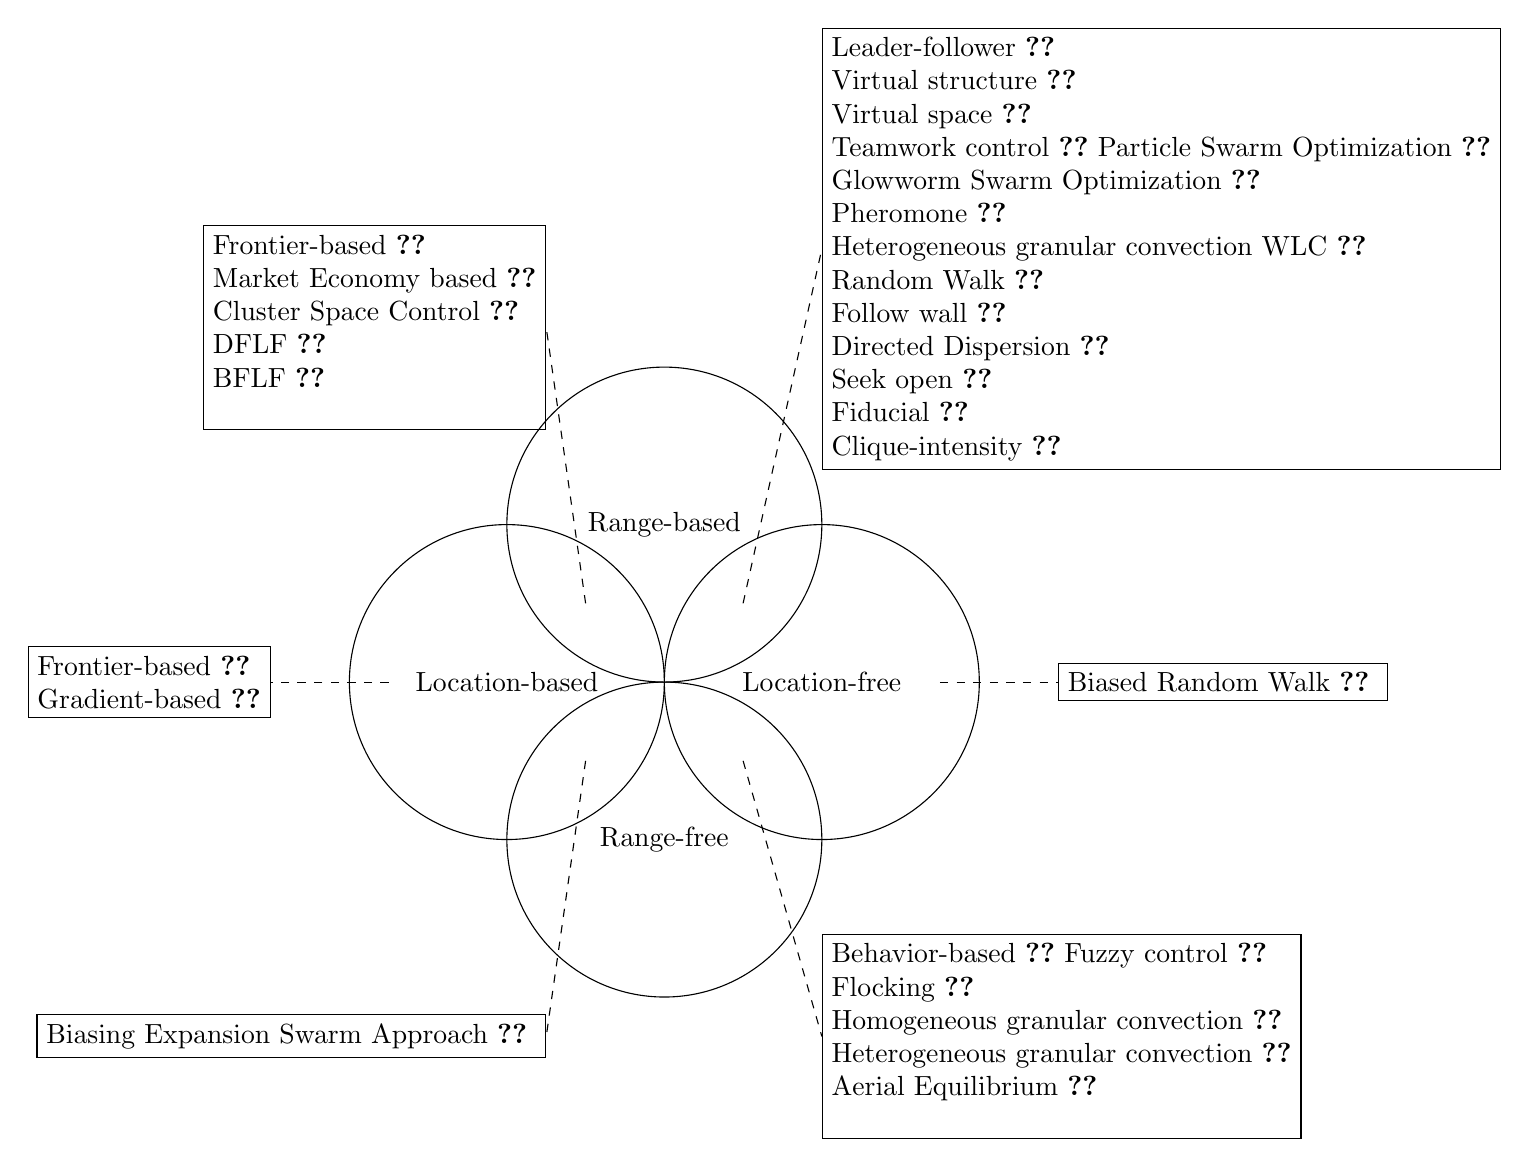
\begin{tikzpicture}
			% standard figures
			\draw \loclb node [text=black] {Location-based};
			\draw \loclf node [text=black] {Location-free};
			\draw \locrb node [text=black] {Range-based};
			\draw \locrf node [text=black] {Range-free};

			% Range-based location-free
			\draw[dashed,-] (1,1) -- (2,5.5) node[anchor=north west] {};
			\node[draw,align=left,anchor=west] at (2,5.5) {
				Leader-follower \ref{sec:Formation}\\
				Virtual structure \ref{sec:Formation}\\
				Virtual space \ref{sec:Formation}\\
				Teamwork control \ref{sec:Formation}
				Particle Swarm Optimization \ref{sec:Localization}\\
				Glowworm Swarm Optimization \ref{sec:Localization}\\
				Pheromone \ref{sec:CollectiveTransport}\\
				Heterogeneous granular convection WLC \ref{sec:CollectiveTransport}\\
				Random Walk \ref{sec:Dispersion}\\
				Follow wall \ref{sec:Dispersion}\\
				Directed Dispersion \ref{sec:Dispersion}\\
				Seek open \ref{sec:Dispersion}\\
				Fiducial \ref{sec:Dispersion}\\
				Clique-intensity \ref{sec:Dispersion}
			};

			% Range-free, location-free
			\draw[dashed,-] (1,-1) -- (2,-4.5) node[anchor=north west] {};
			\node[draw,align=left,anchor=west] at (2,-4.5) {
				Behavior-based \ref{sec:Formation}
				Fuzzy control \ref{sec:Formation}\\
				Flocking \ref{sec:CollectiveTransport}\\
				Homogeneous granular convection \ref{sec:CollectiveTransport}\\
				Heterogeneous granular convection \ref{sec:CollectiveTransport}\\
				Aerial Equilibrium \ref{sec:CollectiveTransport}\\
				%Virtual Pheromone \ref{sec:Path-planning}\\
				%Cardinality \ref{sec:Path-planning}
			};

			% location-free
			\draw[dashed,-] (3.5,0) -- (5,0) node[anchor=north west] {};
			\node[draw,align=left,anchor=west] at (5,0) {
				Biased Random Walk \ref{sec:Localization}
			};

			% location-based
			\draw[dashed,-] (-3.5,0) -- (-5,0) node[anchor=north west] {};
			\node[draw,align=left,anchor=east] at (-5,0) {
				Frontier-based \ref{sec:Exploration}\\
				Gradient-based \ref{sec:Localization}
			};

			% Range-free, location-based
			\draw[dashed,-] (-1,-1) -- (-1.5,-4.5) node[anchor=north west] {};
			\node[draw,align=left,anchor=east] at (-1.5,-4.5) {
				Biasing Expansion Swarm Approach \ref{sec:Localization}
			};

			% Range-based, location-based
			\draw[dashed,-] (-1,1) -- (-1.5,4.5) node[anchor=north west] {};
			\node[draw,align=left,anchor=east] at (-1.5,4.5) {
				Frontier-based \ref{sec:Exploration}\\
				Market Economy based \ref{sec:Exploration}\\
				Cluster Space Control \ref{sec:CollectiveTransport}\\
				DFLF \ref{sec:Dispersion}\\
				BFLF \ref{sec:Dispersion}\\
				%Artificial Bee Colony \ref{sec:Path-planning}\\
				%Multihop Communication \ref{sec:Path-planning}\\
				%Genetic Programming \ref{sec:Path-planning}
			};

			% Range-based
			%\draw[dashed,-] (0,3) -- (0,4.5) node[anchor=north west] {};
			%\node[draw,align=left,anchor=south] at (0,4.5) {

			%};

			% Range-free
			%\draw[dashed,-] (0,-3) -- (0,-4.5) node[anchor=north west] {};
			%\node[draw,align=left,anchor=north] at (0,-4.5) {
			
			%};
		\end{tikzpicture}
    \end{figure}

In the previous sections, we reviewed the main problems found in the field of robotic swarms. 
However, these problems often overlap.
This is because the problems found in this field often consist of multiple different problems. 
We focused on each problem, highlighting the communication methods of every solution and properties of these communication methods. 
We summarize these properties in a Venn-diagram in Figure~\ref{fig:AlgorithmsOverview}, allowing for a compact overview of these solutions.
The algorithms we discussed in previous sections provide useful insight, from which we can derive several conclusions.
Together with the Venn-diagram, we explain how we came to these conclusions. \\


% As can be concluded from the diagram, most algorithms are location-free.
\emph{Location-based} approaches keep track of some kind of map. These approaches are often able to act efficiently and remove redundancy. <<more general advantages??>>
However, a couple of drawbacks can be defined.\\
\\
If an algorithm is \emph{location-based} and \emph{range-based}, the robots can either create some kind of ad-hoc network to have global communication possibilities or accept that they do not have global communication and only share their knowledge with their neighbors.
The first options results in the fact that it is not possible to split up in some way, which takes away one of the great possibilities of robotic swarms, namely to spread out and divide tasks, and can decrease performance.
On the other hand, if we choose the second option, the robots do not have global communication and are not able to share their knowledge of location, for example some kind of map or location history.
\\
In \emph{location-based} and \emph{range-free} algorithms, the robots can either communicate via some central base or not communicate at all. 
In the first case, the performance can be dramatically increased, because of the fact that every robot can have full knowledge of its own and all other location knowledge generated by the robotic swarm, so any redundancy can be removed completely.
However, this will result in very low scalability, since it fully dependent of the capacity of the central base.
If the robots do not communicate at all, but do have knowledge of their location, no real kind of cooperation \todo[inline]{Does this even exist? No communication, but with location?} exists.\\
\\
\emph{Location-free} approaches do not keep track of a map and are only able to determine some kind of relative position to each other or they do not keep track of their location at all. This means they are able to optimally adapt to dynamic environments. <<more general advantages??>>\\
\\
When both \emph{location-free} and \emph{range-free} there in general is no form of coordination. The algorithms in this section are called collective algorithms and are often based on some kind of randomness. These robots all have distributed algorithms and execute the same task. Because there are so many, they will eventually execute a task faster than a single robot.\\
\\
The algorithms that are \emph{location-free} and \emph{range-based} are the algorithms of which we have found the greatest amount. The main reason for this is that the algorithms mentioned in this category are very often highly scalable, have great performance and can be implemented with very simple robots. The robots can either choose to all stay together and share the information they get from their sensors with all of them, but can also choose to spread out in different groups to divide tasks. These algorithms can rather easily be implemented in many real-life applications.\\
\\
Finally, this survey has highlighted some of the main problems that robotic swarms technology has faced in the last few years. Yet we have to acknowledge that some fields have not been discussed in this particular paper. The localization problem, in which robots localize themselves, is used in many algorithms we discussed, but is not mentioned independently. Same goes for target localization, foraging and mapping, although some mapping has been discussed at the exploration problem. In order to get a fully comprehensive view, more research on these topics has to undertaken.

% This makes sense, as location-based are not the most desirable, although they do provide high performance.
% This is mainly because of three reasons. 
% The first reason is cost. 
% When an algorithm is location-based and range-based, the robots used in the swarm generally have to be equipped with advanced sensors. 
% The robots are then more costly in terms of energy consumption and device price, which is not desirable.
% The second reason is scalability. 
% When an algorithm is location-based, in most cases centralized communication is needed. 
% This introduces a lot of overhead, decreasing communication speed when robotic swarms increase in size. 
% The third reason is that algorithms that are location-based can often not be used in dynamic locations, like underwater, space and underground environment.
% This is especially true for algorithms where the operating environment has to be defined beforehand.\\
% \\
% Furthermore we have made the following observation about range usage and location usage. 
% When using a location-free approach, the algorithm easily adapts to dynamic environments.
% A downside to this approach is that the robots in this swarm can not know exactly what absolute location they have.
% This is why some algorithms chooose for a location-based approach. \\
% Some downside is that this approach can require central communication, which makes the scalability relatively low.
% In contrast when using a location-based approach, the robots can very accurately construct solutions out of their absolute location. 
% But, this can often not be implemented in a dynamic environment. 
% When using a location-based approach, we observe very optimal solutions, however these solution only remain to be optimal if the algorithm is used in a static environment. 
% Otherwise some basic algorithms such as collision-detection algorithms have to kick in, which can increase the overall runtime of the algorithm. Range-based algorithms allow for very dynamic environments and is one of the most important approaches due to its extreme usage of distributed intelligence. 

% Range-free algorithms on the other side are not very scalable and do not make use of efficient cooperation.

% This survey only highlighted a few problems that the robotic swarms technology has faced. 

% Thus, more research on this topic needs to be undertaken on additional problems, such as mapping, foraging, target localization and robot localization, in order to create a fully comprehensive overview.

% - voornamelijk location-free
%     - want maps moeten gemerged, bijgehouden worden gedeeld...

% - location-based voornamelijk exploration algoritmes
%     range-free location-free -> goed omdat gebruik bijv van wireless intensity signals erg onnauwkeurig is, non-optimal use of full robotic swarm
%     range-based location-free -> want maps moeten gemerged, bijgehouden worden gedeeld... en dynamische omgeving kan in de gaten gehouden worden
%     range-based -> belangrijkste gedeelte van een swarm, omdat daar de distributed intelligence ligt en dat daar het meeste onderzoek naar gedaan moet worden
%     location-based -> kan ook handig zijn in statische locaties, als er rekening gehouden wordt met de scalability van de swarm  
%     range-free -> matig scalable, maakt niet gebruik van efficiente samenwerking
% - range-based n range-free
